\documentclass[epsfig,10pt,fullpage]{article}

\newcommand{\LabNum}{8}
\newcommand{\CommonDocsPath}{../../../common/docs}
\addtolength{\textwidth}{1.5in}
\addtolength{\oddsidemargin}{-0.75in}
\addtolength{\topmargin}{-0.75in}
\addtolength{\textheight}{1.5in}
\addtolength{\evensidemargin}{0.75in}
\setlength\parindent{0pt}
\raggedbottom

\usepackage{ae,aecompl}
\usepackage{epsfig,float,times}
\usepackage[hypcap]{caption}
\usepackage[pdftex, colorlinks]{hyperref}
\usepackage{graphicx}
\usepackage[usenames, dvipsnames]{color}
\usepackage{rotating}
\usepackage{tikz}
\usetikzlibrary{automata,positioning}
\usepackage{placeins}

\widowpenalty 10000
\clubpenalty 10000

\newcommand{\red}[1]{{\color{red}\sf{#1}}}
\newcommand{\green}[1]{{\color{green}\sf{#1}}}
\newcommand{\blue}[1]{{\color{blue}\sf{#1}}}
\definecolor{PineGreen}{rgb}{0.0, 0.47, 0.44}
\definecolor{ForestGreen}{rgb}{0.13, 0.55, 0.13}
\definecolor{Brown}{rgb}{0.59, 0.29, 0.0}

\newcommand{\UPDatePublished}{Oct 2021}
\newcommand{\versnum}{21.1} %version number quartus/AMP
\newcommand{\quartusname}{Quartus\textsuperscript{\textregistered} Prime}	
\newcommand{\UPTextBar}{For \quartusname{} \versnum{}}
\newcommand{\thisyear}{2021 } %for copyright
\newcommand{\company}{FPGAcademy.org}
\newcommand{\longteamname}{FPGAcademy.org}
\newcommand{\teamname}{FPGAcademy}
\newcommand{\website}{FPGAcademy.org}

\newcommand{\productAcronym}{AMP}
\newcommand{\productNameShort}{Monitor Program}

\newcommand{\productNameMedTM}{A Monitor Program}
\newcommand{\productNameMed}{A Monitor Program}

%\newcommand{\headerLogoFilePath}[1]{#1/FPGAcademy.png}

% listings is a package that supports encapsulating source code in LaTeX conveniently
\usepackage{listings}

\def\expandparam\lstinputlisting[#1]#2{\edef\tmp{\noexpand\lstinputlisting[#1]{#2}}\tmp}

%%%%%%%%%%%%%%%%%%%% Source Code Formatting %%%%%%%%%%%%%%%%%%%%
\definecolor{globalCommentColour}{rgb}{0.588,0.588,0.588}

%%%%%%%%%%%%%%%%%%%%%%%%%%%%%%%%%%%%%%%%%%%%%%%%%%%%
% Defining language style
% NiosII ASM
\lstdefinelanguage[NiosII]{Assembler} {
  morekeywords={add, addi, and, andhi, andi, beq, bge, bgeu, bgt, bgtu, ble,  bleu, blt, bltu, bne, br, break,
  bret, call, callr, cmpeq, cmpeqi, cmpge, cmpgei, cmpgeu, cmpgeui, cmpgt, cmpgti, cmpgtu, cmpgtui, cmple,
  cmplei, cmpleu, cmpleui, cmplt, cmplti, cmpltu, cmpltui, cmpne, cmpnei, custom, div, divu, eret, flushd,
  flushda, flushi, flushp, initd, initda, initi, jmp, jmpi, ldb, ldbio, ldbu, ldbuio, ldh, ldhio, ldhu, ldhuio,
  ldw, ldwio, mov, movhi, movi, movia, movui, mul, muli, mulxss, mulxsu, mulxuu, nextpc, nop, nor, or, orhi, ori,
  rdctl, rdprs, ret, rol, roli, ror, sll, slli, sra, srai, srl, srli, stb, stbio, sth, sthio, stw, stwio,
  sub, subi, sync, trap, wrctl, wrtcl, wrprs, xor, xori, xorhi, xori},
  morekeywords=[2]{.abort, .ABORT, .align, .app-file, .ascii, .asciz, .balign, .byte, .comm, .data, .def,
  .desc, .dim, .double, .eject, .else, .end, .endef, .endif, .equ, .equiv, .err, .extern, .file, .fill, .float,
  .global, .globl, .hword, .ident, .if, .include, .int, .irp, .irpc, .lcomm, .lflags, .line, .linkonce, .ln,
  .list, .long, .macro, .mri, .nolist, .octa, .org, .p2align, .psize, .quad, .rept, .sbttl, .scl, .section,
  .set, .short, .single, .size, .sleb128, .skip, .space, .stadb, .stabn, .stabs, .string, .symver, .tag,
  .text, .title, .type, .val, .uleb128, .word},
  morekeywords=[3]{et, bt, gp, sp, fp, ea, sstatus, ra, pc, status, estatus, bstatus, ienable, ipending, cpuid,
  exception, pteaddr, tlbacc, tlbmisc, eccinj, badaddr, config, mpubase, mpuacc},
  sensitive=t,
  alsoletter=.,
  morestring=[b]",
  morecomment=[s]{/*}{*/},
  morecomment=[l]\#,
}[keywords,comments,strings]
   
%% NOTE: morekeywords=[2] are GNU directives.
   
\definecolor{niosInstructionColour}{rgb}{0.000,0.608,0.000}
\definecolor{niosDirectiveColour}{rgb}{0.000,0.000,0.902}
\definecolor{niosSpecialRegColour}{rgb}{0.000,0.000,0.000}
\definecolor{niosStringColour}{rgb}{0.808,0.482,0.000}
   
%% NOTE: To make bold use: =\bfseries\color{<colour>}
\lstdefinestyle{defaultNiosStyle} {
  language=[NiosII]{Assembler},
  stringstyle=\color{niosStringColour},
  keywordstyle=\color{niosInstructionColour},
  keywordstyle=[2]\color{niosDirectiveColour},
  keywordstyle=[3]\itshape\color{niosSpecialRegColour}
}
%%%%%%%%%%%%%%%%%%%%%%%%%%%%%%%%%%%%%%%%%%%%%%%%%%%%

%%%%%%%%%%%%%%%%%%%%%%%%%%%%%%%%%%%%%%%%%%%%%%%%%%%%
% Defining language style
% ArmA9 ASM
\lstdefinelanguage[ArmA9]{Assembler} {
  morekeywords={ADC, ADD, ADDS, AND, ANDS, B, BAL, BEQ, BGE, BGT, BL, BLT, BIC, BKPT, BLX, BNE, BX, CDP, CLZ, CMN, CMP, EOR,
  EORS, LDC, LDM, LDR, LDRB, LDRBT, LDRH, LDRSB, LDRSH, LDRT, LSL, MCR, MLA, MOV, MOVW, MOVT, MRC, MRS, MSR, MUL, MVN, ORR, PLD,
  ROR, RSB, RSC, SBC, SMLAL, SMULL, STC, STM, STR, STRB, STRBT, STRH, STRT, SUB, SUBS, SWI, SWP, SWPB, TEQ, UMLAL,
  PUSH, POP, MOVS, RORS, LSR},
  morekeywords=[2]{.abort, .ABORT, .align, .app-file, .ascii, .asciz, .balign, .byte, .comm, .data, .def,
  .desc, .dim, .double, .eject, .else, .end, .endef, .endif, .equ, .equiv, .err, .extern, .file, .fill, .float,
  .global, .globl, .hword, .ident, .if, .include, .int, .irp, .irpc, .lcomm, .lflags, .line, .linkonce, .ln,
  .list, .long, .macro, .mri, .nolist, .octa, .org, .p2align, .psize, .quad, .rept, .sbttl, .scl, .section,
  .set, .short, .single, .size, .sleb128, .skip, .space, .stadb, .stabn, .stabs, .string, .symver, .tag,
  .text, .title, .type, .val, .vectors, .uleb128, .word},
  morekeywords=[3]{SP, PC, MIDR, CTR, TCMTR, TLBTR, MPIDR, ID_PFR0, ID_PFR1, ID_DFR0, ID_MMFR0, ID_MMFR1, ID_MMFR2,
  ID_MMFR3, ID_ISAR0, ID_ISAR1, ID_ISAR2, ID_ISAR3, ID_ISAR4, CCSIDR, CLIDR, AIDR, CSSELR, TTBR0, TTRB1, TTBR2, DACR,
  DFSR, IFSR, ADFSR, AIFSR, DFAAR, IFAR, ICIALLUIS, BPIALLIS, PAR, ICIALLU, ICIMVAU, BPIALL, DCIMVAC, DCISW, V2PCWPR,
  DCCVAC, DCCSW, DDIMVAC, DCISW, TLBALLIS, TLBIMVAIS, TLBIASIDIS, TLBIMVAAIS, TLBIALL, TLBIMVA, TLBIASID, TLBIMVAA,
  PMCR, PMCNTENSET, PMCNTENCLR, PMOVSR, PMSWINC, PMSELR, PMXEVTYPER, PMXEVCNTR, PMUSERENR, PMINTENSET, PMINTENCLR,
  PRRR, NRRR, PLEIDR, PLEASR, PLEFSR, PLEUAR, PLEPCR, VBAR, MVBAR, ISR, FCSEIDR, CONTEXTIDR, TPIDRURW, TPIDRURO, TPIDRPRW},
  sensitive=f,
  alsoletter=.,
  morestring=[b]",
  morecomment=[s]{/*}{*/},
  morecomment=[l]{//},
}[keywords,comments,strings]
   
%% NOTE: morekeywords=[2] are GNU directives.
   
\definecolor{armInstructionColour}{rgb}{0.000,0.608,0.000}
\definecolor{armDirectiveColour}{rgb}{0.000,0.000,0.902}
\definecolor{armSpecialRegColour}{rgb}{0.000,0.000,0.000}
\definecolor{armStringColour}{rgb}{0.808,0.482,0.000}
   
\lstdefinestyle{defaultArmStyle} {
  language=[ArmA9]{Assembler},
  stringstyle=\color{armStringColour},
  keywordstyle=\color{armInstructionColour},
  keywordstyle=[2]\color{armDirectiveColour},
  keywordstyle=[3]\itshape\color{armSpecialRegColour}
}
%%%%%%%%%%%%%%%%%%%%%%%%%%%%%%%%%%%%%%%%%%%%%%%%%%%%

%%%%%%%%%%%%%%%%%%%%%%%%%%%%%%%%%%%%%%%%%%%%%%%%%%%%
% Defining language style
% FPGAcademy ASM
\lstdefinelanguage{ASM}{
  morekeywords = [1]{mv, mvt, mvne, mvcc, add, sub, st, ld, and, b, bne, beq, bcc, bcs},
  morekeywords = [2]{word, define},
  keywordstyle = [1]\color{ForestGreen},
  keywordstyle = [2]\color{blue},
  sensitive = true,
  morecomment = [l]{//},
}

\lstset{
  language = ASM,
  basicstyle=\small\color{black}\ttfamily,
  commentstyle=\small\color{Brown}\itshape\ttfamily,
  showstringspaces=false,
  frame=none, %lines % boxed listings
  breaklines=true,
  breakatwhitespace=true,
  tabsize=3
}
%%%%%%%%%%%%%%%%%%%%%%%%%%%%%%%%%%%%%%%%%%%%%%%%%%%%

%%%%%%%%%%%%%%%%%%%%%%%%%%%%%%%%%%%%%%%%%%%%%%%%%%%%
% Defining language style
% Java
\definecolor{javaStringColour}{rgb}{0.808,0.482,0}
%%%%%%%%%%%%%%%%%%%%%%%%%%%%%%%%%%%%%%%%%%%%%%%%%%%%

%%%%%%%%%%%%%%%%%%%%%%%%%%%%%%%%%%%%%%%%%%%%%%%%%%%%
% Defining language style
% C
\definecolor{CStringColour}{rgb}{0.808,0.482,0}

\lstset{
  language = C,
  basicstyle=\small\color{black}\ttfamily, 
  commentstyle=\small\color{PineGreen}\itshape\ttfamily,
  keywordstyle=\small\color{blue}\bfseries\ttfamily,
  showstringspaces=false,
  frame=none, %lines % boxed listings
  breaklines=true,
  breakatwhitespace=true,
  tabsize=3
}
%%%%%%%%%%%%%%%%%%%%%%%%%%%%%%%%%%%%%%%%%%%%%%%%%%%%

%%%%%%%%%%%%%%%%%%%%%%%%%%%%%%%%%%%%%%%%%%%%%%%%%%%%
% Defining language style
% Verilog
\definecolor{verilogCommentColour}{rgb}{0.000,0.502,0.000}

\lstdefinestyle{defaultVerilogStyle} {
  language={Verilog},
  keywordstyle=\color{blue},
  commentstyle=\color{verilogCommentColour}
}
%%%%%%%%%%%%%%%%%%%%%%%%%%%%%%%%%%%%%%%%%%%%%%%%%%%%

%%%%%%%%%%%%%%%%%%%%%%%%%%%%%%%%%%%%%%%%%%%%%%%%%%%%
% Defining language style
% VHDL
\lstdefinestyle{defaultVHDLStyle} {
  language={VHDL},
  keywordstyle=\color{blue},
  commentstyle=\color{verilogCommentColour}
}
%%%%%%%%%%%%%%%%%%%%%%%%%%%%%%%%%%%%%%%%%%%%%%%%%%%%

%%%%%%%%%%%%%%%%%%%%%%%%%%%%%%%%%%%%%%%%%%%%%%%%%%%%
% Defining language style
% LaTeX
\lstdefinelanguage[LocalLaTeX]{TeX}[LaTeX]{TeX}{moretexcs={bf, it, sf, lstset},}

\lstdefinestyle{defaultLocalLatexStyle} {
  language=[LocalLatex]{TeX},
  keywordstyle=\color{blue}\bfseries,
  keywordstyle=[2]\color{blue},
  keywordstyle=[3]\color{blue}\bfseries
}
%%%%%%%%%%%%%%%%%%%%%%%%%%%%%%%%%%%%%%%%%%%%%%%%%%%%

%%%%%%%%%%%%%%%%%%%%%%%%%%%%%%%%%%%%%%%%%%%%%%%%%%%%
% Defining language style
% Default
\lstset{
  basicstyle=\small\color{black}\ttfamily,
  commentstyle=\small\color{globalCommentColour}\itshape\ttfamily,
  keywordstyle=\small\color{blue}\bfseries\ttfamily,
  showstringspaces=false,
  frame=none, %lines % boxed listings
  breaklines=true,
  breakatwhitespace=true,
  tabsize=3
}
%%%%%%%%%%%%%%%%%%%%%%%%%%%%%%%%%%%%%%%%%%%%%%%%%%%%


\hypersetup{
  pdftitle={Digital Logic Lab Exercise \LabNum},
  linkcolor=blue,
  hyperindex=true,
  pdfauthor={FPGAcademy.org},
  pdfkeywords={FPGAcademy.org, FPGAcademy, Lab, Exercise, Digital Logic},
  bookmarks,
  bookmarksopen=false,
  filecolor=blue,
  pdfstartview={FitH},
  urlcolor=blue,
  plainpages=false,
  pdfpagelabels=true,
  linkbordercolor={1 1 1} %no color for link border
}



\begin{document}

\centerline{\huge Digital Logic}
~\\
\centerline{\huge Laboratory Exercise \LabNum}
~\\
\centerline{\large Memory Blocks}
~\\

In computer systems it is necessary to provide a substantial amount of memory.
If a system is implemented using FPGA technology it is possible
to provide some amount of memory by using the memory resources that exist
in the FPGA device.  In this exercise we will examine the general issues involved in 
implementing such memory.

~\\
A diagram of the random access memory (RAM) module that we will implement is shown in Figure~\ref{fig:fig1}{\it a}. It contains 32 four-bit words (rows), which are accessed using a five-bit
{\it address} port, a four-bit {\it data} port, and a {\it write} control input.

~\\
The FPGAs that are included on the Intel\textsuperscript{\textregistered} FPGA DE10-Lite, DE0-CV, DE1-SoC, and DE2-115 boards 
provide dedicated memory resources.  The MAX\textsuperscript{\textregistered} 10 FPGA on the DE10-Lite, and Cyclone\textsuperscript{\textregistered} IV FPGA
on the DE2-115 contain dedicated memory resources called {\it M9K blocks}. The Cyclone V FPGA 
on the DE0-CV and DE1-SoC boards have {\it M10K blocks}. Each M9K block contains 9216 memory 
bits, while each M10K block contains 10240 memory bits. Both M9K and M10k blocks can be 
configured to implement memories of various sizes. A common term used to specify the size of 
a memory is its {\it aspect ratio}, which gives the {\it depth} in words and the {\it width} 
in bits (depth {\sf x} width). In this exercise we will use an aspect ratio that is four
bits wide, and we will use only the first 32 words in the memory. Although the M9K and M10K 
blocks support many other modes of operation, we will not discuss them here.

\begin{figure}[H]
	\begin{center}
		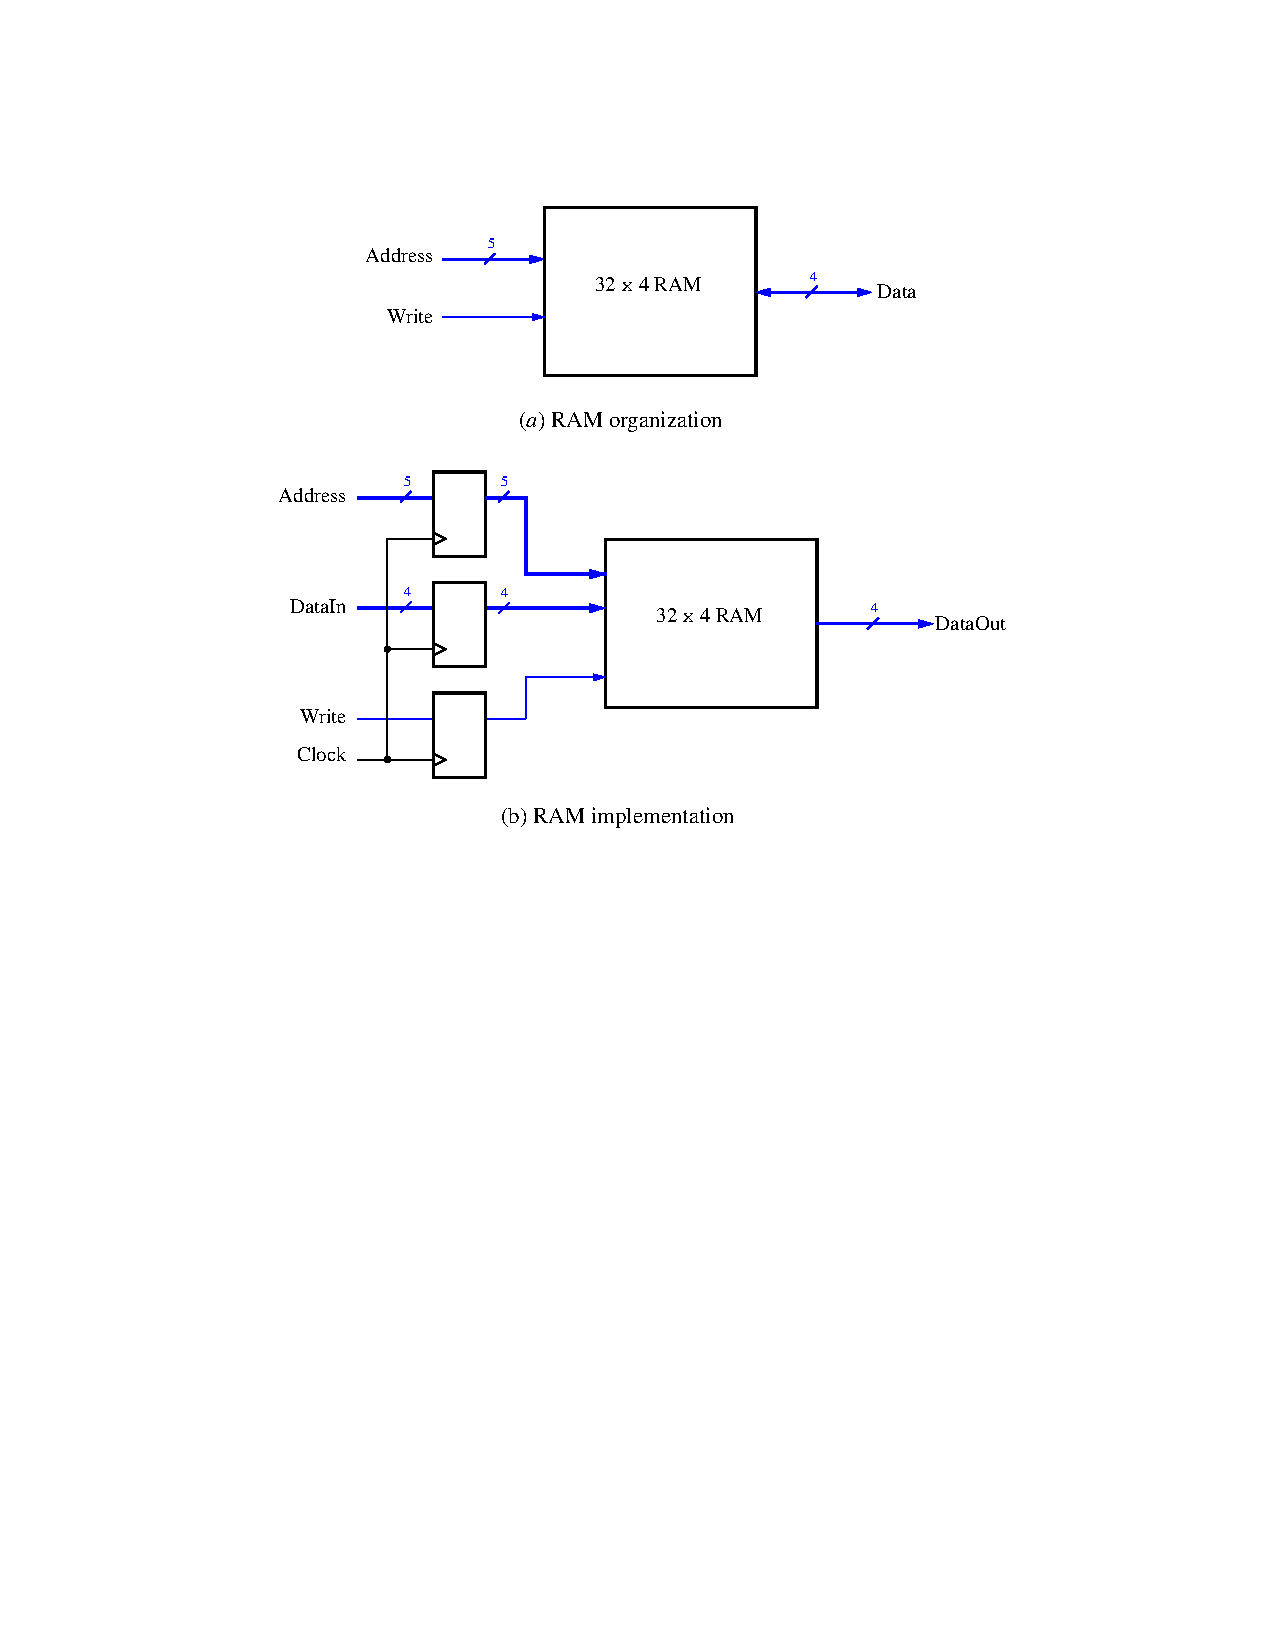
\includegraphics[]{figures/figure1.pdf}
	\end{center}
	\caption{A 32 {\sf x} 4 RAM module.}
	\label{fig:fig1}
\end{figure}

There are two important features of the M9K and M10K blocks that have to be mentioned.
First, they includes registers that can be used to synchronize all of the 
input and output signals to a clock input. The registers on the input ports must always be
used, and the registers on the output ports are optional.  Second, the blocks have separate
ports for data being written to the memory and data being read from the memory. 
Given these requirements, we will implement the modified 32 {\sf x} 4 RAM module shown in 
Figure~\ref{fig:fig1}{\it b}. It includes registers for the {\it address}, {\it data input}, 
and {\it write} ports, and uses a separate unregistered {\it data output} port.

\section*{Part I}
\addcontentsline{toc}{1}{Part I}
Commonly used logic structures, such as adders, registers, counters and memories, 
can be implemented in an FPGA chip by using prebuilt modules that are provided in 
{\it libraries}.  In this exercise we will use such a module to implement the memory 
shown in Figure~\ref{fig:fig1}$b$.

\begin{enumerate}
\item Create a new Quartus\textsuperscript{\textregistered} project to implement the memory module.

\item To open the IP Catalog in the Quartus software click on {\sf Tools} $>$ {\sf IP Catalog}. 
In the IP Catalog window choose the {\it RAM:~1-PORT} module, which is found under 
the {\sf Basic Functions $>$  On Chip Memory} category.  Select {\sf VHDL} as the type 
of output file to create, give the file the name {\it ram32x4.vhd}, and click {\sf OK}. 
As shown in Figure~\ref{fig:fig2} specify a memory size of 32 four-bit words. Select M9K if 
your DE-series board has a MAX 10 or Cyclone IV FPGA, otherwise select M10K. 
Also on this screen accept the default setting to use a single clock for the memory's registers,
and then advance to the page shown in Figure~\ref{fig:fig3}. On this page {\it deselect} the 
setting called {\sf 'q' output port} under the category {\sf Which ports should be registered?}.
This setting creates a RAM module that matches the structure in Figure~\ref{fig:fig1}{\it b}, 
with registered input ports and unregistered output ports. Accept defaults for the rest of 
the settings in the Wizard, and click the {\sf Finish} button to exit from this tool.  Examine the 
{\it ram32x4.vhd} VHDL file which defines the following subcircuit:

\begin{center}
\begin{tabbing}
ENTITY ram32x4 IS\\
ZZ\=PORT ~( \=addressZZ \=: OUTZ\=STD\_LOGIC;\kill
\>PORT ( \>address \>: IN \>STD\_LOGIC\_VECTOR (4 DOWNTO 0);\\
\>\>clock \>: IN \>STD\_LOGIC  := '1';\\
\>\>data	\>: IN \>STD\_LOGIC\_VECTOR (3 DOWNTO 0);\\
\>\>wren	\>: IN \>STD\_LOGIC ;\\
\>\>q	\>: OUT \>STD\_LOGIC\_VECTOR (3 DOWNTO 0) );\\
END ram32x4;\\
\end{tabbing}
\end{center}

\item Instantiate this subcircuit in a top-level VHDL file that includes appropriate input and 
output signals for the memory ports given in Figure~\ref{fig:fig1}{\it b}.
\item Compile the circuit. Observe in the Compilation Report that the Quartus 
Compiler uses 128 bits in one of the FPGA memory blocks to implement the RAM circuit.
\item Simulate the behavior of your circuit using Modelsim and ensure that you can read and write data in
the memory. Use the included testbench file as a baseline for your simulation inputs.
An example simulation output is given in Figure~\ref{fig:figsim}.
\end{enumerate}

\begin{figure}[H]
	\begin{center}
		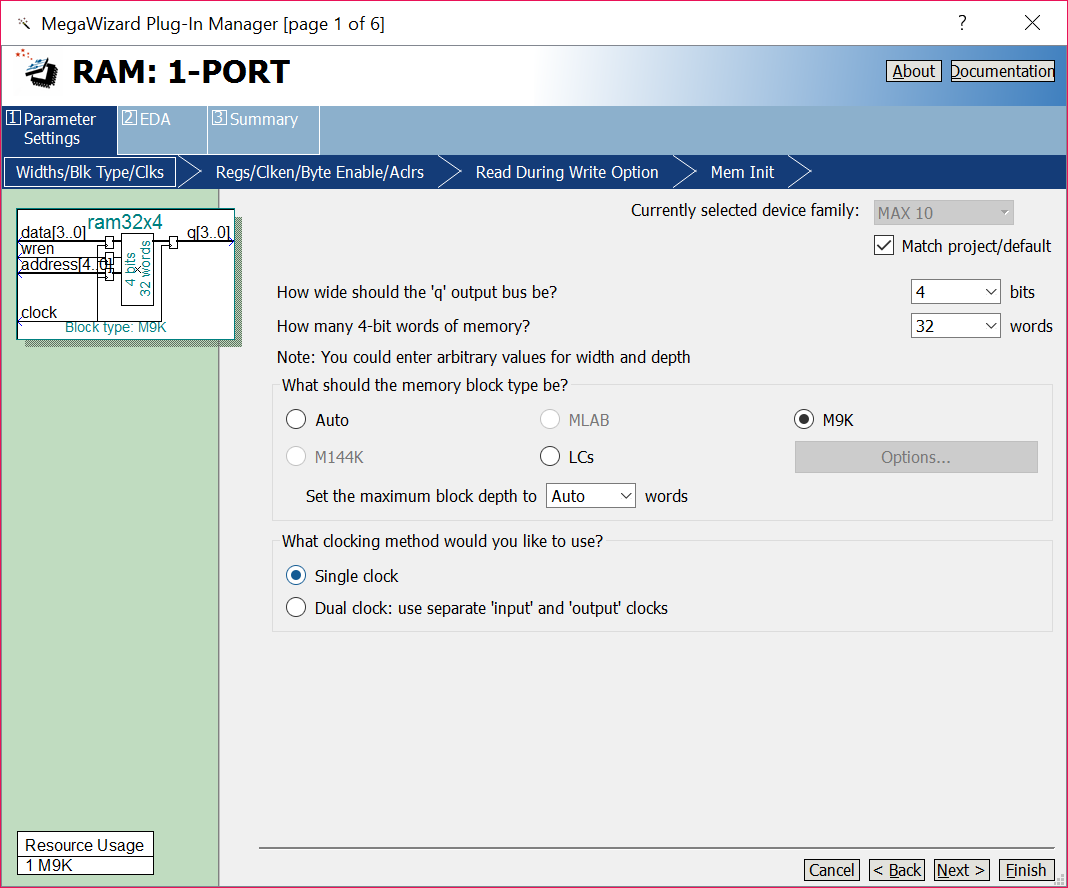
\includegraphics[scale=0.42]{figures/figure2.png}
	\end{center}
	\caption{Configuring the size of the memory module.}
	\label{fig:fig2}
\end{figure}

\begin{figure}[H]
	\begin{center}
		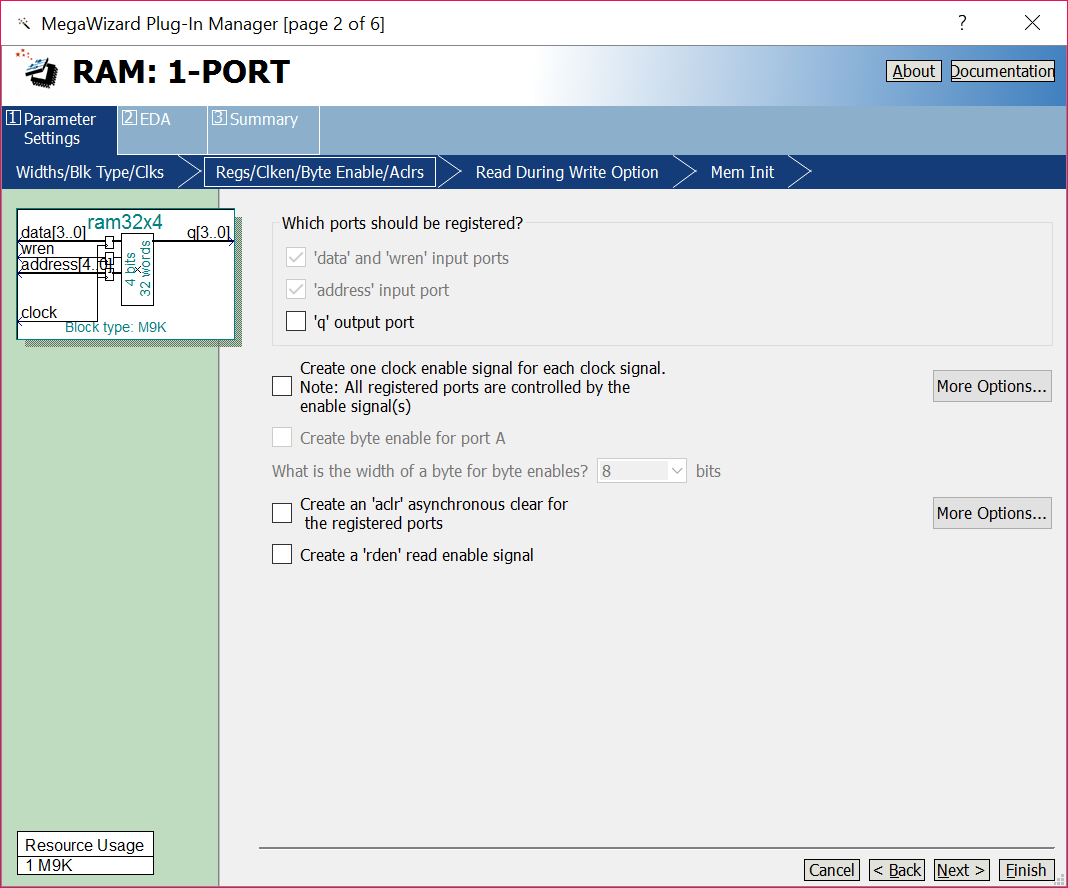
\includegraphics[scale=0.42]{figures/figure3.png}
	\end{center}
	\caption{Configuring input and output ports.}
	\label{fig:fig3}
\end{figure}

\begin{figure}[H]
	\begin{center}
		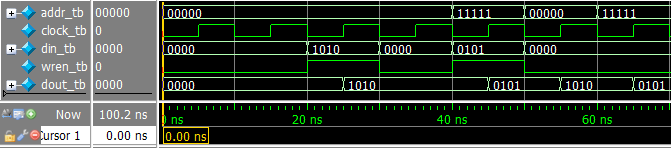
\includegraphics[scale=0.8]{figures/simulation.png}
	\end{center}
	\caption{An example of simulation output.}
	\label{fig:figsim}
\end{figure}

\section*{Part II}
\addcontentsline{toc}{2}{Part II}
Now, we want to realize the memory circuit in the FPGA on your DE-series board, and 
use slide switches to load some data into the created memory. 
We also want to display the contents of the RAM on the 7-segment displays.
\begin{enumerate}
\item Make a new Quartus project which will be used to 
implement the desired circuit on your DE-series board.
\item Create another VHDL file that instantiates the {\it ram32x4} module and that
includes the required input and output pins on your DE-series board. 
Use slide switches {\it SW}$_{3-0}$ to provide input data for
the RAM, and use switches switches {\it SW}$_{8-4}$ to specify the address. 
Use {\it SW}$_{9}$ as the {\it Write} signal and use {\it KEY}$_0$ as the {\it Clock} input. 
Show the address value on the 7-segment displays {\it HEX}$5-4$, show the
data being input to the memory on {\it HEX}2, and show the data read out
of the memory on {\it HEX}0. 
\item Test your circuit and make sure that data can be stored into the memory at various
locations.
\end{enumerate}

\section*{Part III}
\addcontentsline{toc}{3}{Part III}
Instead of creating a memory module subcircuit by using the IP Catalog, we can implement the 
required memory by specifying its structure in VHDL code.
In a VHDL-specified design it is possible to define the memory as a
multidimensional array. A 32 {\sf x} 4 array, which has 32 words with
4 bits per word, can be declared by the statement

\begin{center}
\begin{minipage}[t]{12.5 cm}
\begin{tabbing}
TYPE mem IS ARRAY(0 TO 31) OF STD\_LOGIC\_VECTOR(3 DOWNTO 0);\\
SIGNAL memory\_array : mem;
\end{tabbing}
\end{minipage}
\end{center}

In an FPGA such an array can be implemented either by using
the flip-flops that each logic element contains or, more efficiently, 
by using the built-in memory blocks.
The Quartus Help provides other examples of VHDL code 
that show how memory can be specified (search in the Help for ``Inferred memory''). 

~\\
Perform the following steps:

\begin{enumerate}
\item Create a new project which will be used to implement the desired
circuit on your DE-series board.
\item Write a VHDL file that provides the necessary functionality,
including the ability to load the RAM and read its contents as was done in
Part II.
\item Assign the pins on the FPGA to connect to the switches and the 
7-segment displays.
\item Compile the circuit and download it into the FPGA chip.
\item Test the functionality of your design by applying some inputs
and observing the output.
\end{enumerate}

\section*{Part IV}
\addcontentsline{toc}{4}{Part IV}
The SRAM block in Figure~\ref{fig:fig1} has a single port that provides the address for 
both read and write operations. For this part you will create a different type of memory module,
in which there is one port for supplying the address for a read operation, and a separate
port that gives the address for a write operation. Perform the following steps.

\begin{enumerate}
\item Create a new Quartus project for your circuit. To generate the desired memory
module open the IP Catalog and select the {\it RAM: 2-PORT} module in the 
{\sf Basic Functions $>$  On Chip Memory} category. As shown in Figure~\ref{fig:fig4}, 
choose {\sf With one read port and one write port} in the category called {\sf How will 
you be using the dual port ram?}

Configure the memory size, clocking method, and registered ports the same way as Part II.
As shown in Figure~\ref{fig:fig5} select {\sf I do not care (The outputs will be undefined)} 
for {\sf Mixed Port Read-During-Write for Single Input Clock RAM}.
This setting specifies that it does not matter whether the memory outputs the new data being 
written, or the old data previously stored, in the case that the write and read addresses are 
the same during a write operation.

Figure~\ref{fig:fig6} shows how the memory words can be initialized to specific values. It 
makes use of a feature that allows the memory module to be loaded with data when the circuit is
programmed into the FPGA chip. As shown in the figure, choose the setting {\sf Yes, use this
file for the memory content data}, and specify the filename {\it ram32x4.mif}. An example
of a {\it MIF} file is provided in Figure~\ref{fig:mif}. You can also learn
about the format of a {\it memory initialization file} (MIF) by using the Quartus Help.
You will need to create a MIF file like the one in Figure~\ref{fig:mif} to test your circuit.
Finish the Wizard and then examine the generated memory module in the file {\it ram32x4.vhd}.

\item Write a VHDL file that instantiates your dual-port memory. 
To see the RAM contents, add to your design a capability to display the
content of each four-bit word (in hexadecimal format) on the 7-segment display
{\it HEX}0. Use a counter as a read address, and scroll through the memory locations 
by displaying each word for about one second. As each word is being displayed, show its 
address (in hex format) on the 7-segment displays {\it HEX}$3-2$. Use the 50 MHz 
clock, {\it CLOCK\_50}, and use {\it KEY}$_0$ as a reset input. For 
the write address and corresponding data use switches {\it SW}$_{8-4}$ and {\it SW}$_{3-0}$.
Show the write address on {\it HEX}$5-4$ and show the write data on {\it HEX}1.
Make sure that you properly synchronize the slide switch inputs to the 50 MHz clock signal.

\item Test your circuit and verify that the initial contents of the memory match
your {\it ram32x4.mif} file. Make sure that you can independently write data to any
address by using the slide switches.
\end{enumerate}

\begin{figure}[H]
	\begin{center}
		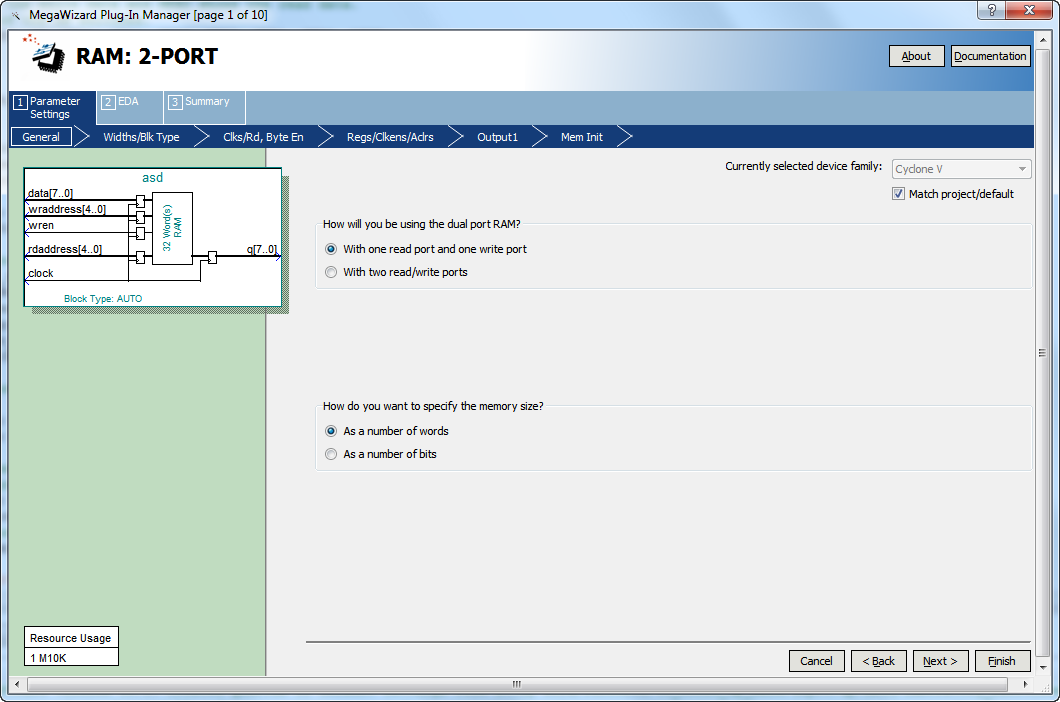
\includegraphics[scale=0.50]{figures/figure4.png}
	\end{center}
	\caption{Configuring the two input ports of the RAM.}
	\label{fig:fig4}
\end{figure}

\begin{figure}[H]
	\begin{center}
		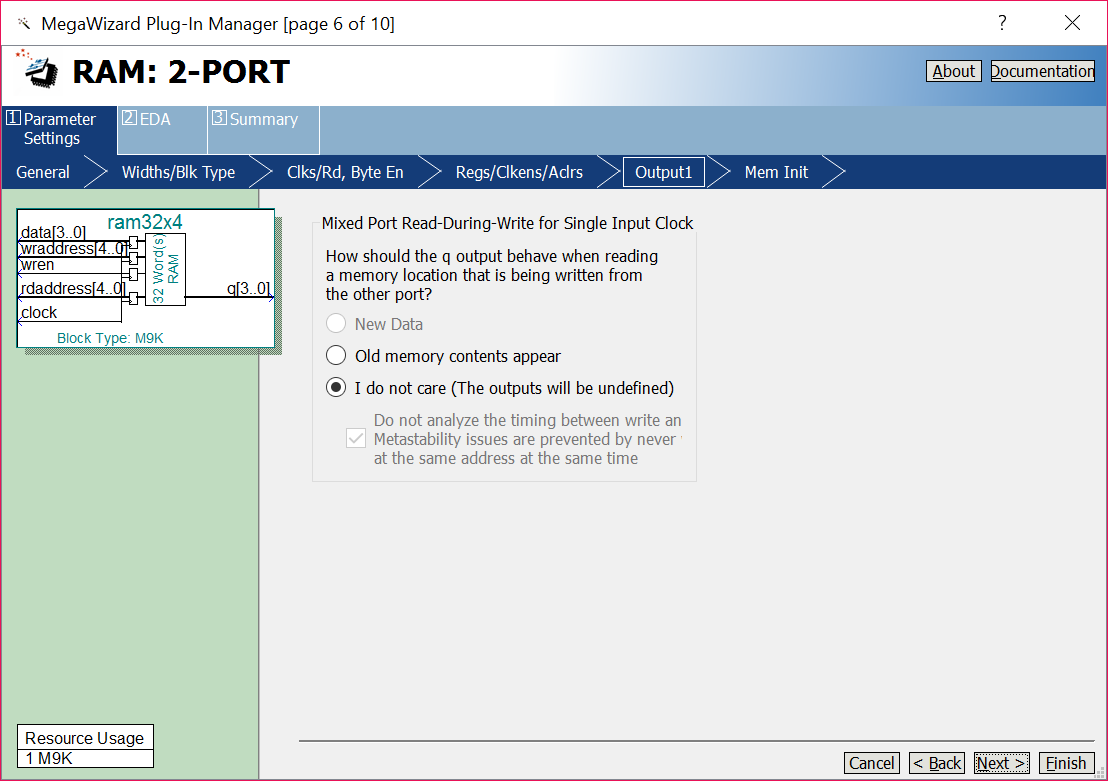
\includegraphics[scale=0.50]{figures/figure5.png}
	\end{center}
	\caption{Configuring the output of the RAM when reading and writing to the same address.}
	\label{fig:fig5}
\end{figure}

\begin{figure}[H]
	\begin{center}
		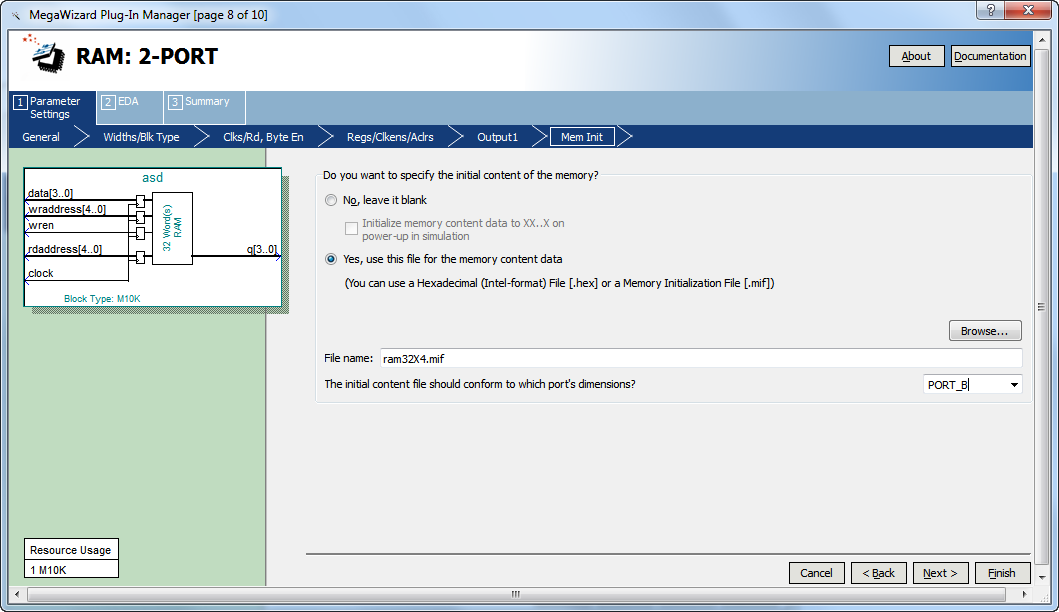
\includegraphics[scale=0.50]{figures/figure6.png}
	\end{center}
	\caption{Specifying a memory initialization file (MIF).}
	\label{fig:fig6}
\end{figure}

\begin{figure}[H]
\begin{center}
\begin{minipage}[t]{12.5 cm}
\begin{tabbing}
{\bf DEPTH} = 32;\\
{\bf WIDTH} = 4;\\
{\bf ADDRESS\_RADIX} = HEX;\\
{\bf DATA\_RADIX} = BIN;\\
{\bf CONTENT}\\
{\bf BEGIN}\\
\\
0 : 0000;\\
1 : 0001;\\
2 : 0010;\\
3 : 0011;\\
$\ldots$ (some lines not shown)\\
1E : 1110;\\
1F : 1111;\\
\\
{\bf END};\\
\end{tabbing}
\end{minipage}
\end{center}
\caption{An example memory initialization file (MIF).}
\label{fig:mif}
\end{figure}


%%%%%%%%%%%%%%%%%%%%%%%%%%%%%%%%%%%%%%%%
%%% FPGAcademy Copyright Information %%%
%%%%%%%%%%%%%%%%%%%%%%%%%%%%%%%%%%%%%%%%

%Always put the copyright on a new page (clear page), with some vertical space from top
\clearpage
\vspace{1in}

\noindent

Copyright {\copyright} FPGAcademy.org. All rights reserved. FPGAcademy and the 
FPGAcademy logo are trademarks of FPGAcademy.org.  This document is provided 
"as is", without warranty of any kind, express or implied, including but not 
limited to the warranties of merchantability, fitness for a particular purpose 
and noninfringement. In no event shall the authors or copyright holders be 
liable for any claim, damages or other liability, whether in an action of 
contract, tort or otherwise, arising from, out of or in connection with the 
document or the use or other dealings in the document.
~\\
~\\
**Other names and brands may be claimed as the property of others.


\end{document}
 
